\documentclass[aspectratio=169, 11pt]{beamer}
% ============================================================================
% Preambulo compartido para presentaciones Beamer
% Estadistica 2026-II - Pontificia Universidad Javeriana
% Incluir con: % ============================================================================
% Preambulo compartido para presentaciones Beamer
% Estadistica 2026-II - Pontificia Universidad Javeriana
% Incluir con: % ============================================================================
% Preambulo compartido para presentaciones Beamer
% Estadistica 2026-II - Pontificia Universidad Javeriana
% Incluir con: \input{../preambulo_beamer.tex} despues de \documentclass
% ============================================================================

\usepackage[T1]{fontenc}
\usepackage[utf8]{inputenc}
\usepackage[spanish]{babel}
\usepackage{amsmath, amssymb, amsfonts}
\usepackage{booktabs}
\usepackage{graphicx}
\usepackage{tikz}
\usetikzlibrary{shapes.geometric, positioning, arrows.meta, calc}
\usepackage{pgfplots}
\pgfplotsset{compat=1.18}
\usepackage{listings}
\usepackage{xcolor}
\usepackage{hyperref}
\usepackage{multicol}


% --- Tema Beamer (minimalista) ---
\usetheme{default}
\usecolortheme{default}
\usefonttheme{default}
\setbeamertemplate{navigation symbols}{}
\setbeamertemplate{caption}[numbered]
\setbeamertemplate{footline}{%
  \hfill\usebeamerfont{footline}\insertframenumber/\inserttotalframenumber\hspace{1em}\vspace{0.5em}%
}
\setbeamertemplate{itemize items}[circle]
\setbeamertemplate{enumerate items}[default]

% --- Colores institucionales (sutiles) ---
\definecolor{javeriana}{RGB}{0, 62, 105}
\definecolor{javerianalight}{RGB}{0, 105, 170}
\definecolor{codigobg}{RGB}{245, 245, 245}
\definecolor{codigofg}{RGB}{40, 40, 40}
\definecolor{comentario}{RGB}{100, 100, 100}
\definecolor{keyword}{RGB}{0, 100, 150}
\definecolor{string}{RGB}{180, 60, 30}

\setbeamercolor{title}{fg=javeriana}
\setbeamercolor{frametitle}{fg=javeriana}
\setbeamercolor{structure}{fg=javeriana}
\setbeamercolor{block title}{fg=white, bg=javeriana!75}
\setbeamercolor{block body}{bg=javeriana!5}
\setbeamercolor{block title alerted}{fg=white, bg=red!70!black}
\setbeamercolor{block body alerted}{bg=red!5}
\setbeamercolor{block title example}{fg=white, bg=green!40!black}
\setbeamercolor{block body example}{bg=green!5}
\setbeamercolor{item}{fg=javeriana}

\setbeamerfont{title}{series=\bfseries, size=\Large}
\setbeamerfont{frametitle}{series=\bfseries}

% --- Configuracion de listings para R ---
\lstset{
  language=R,
  basicstyle=\ttfamily\footnotesize,
  backgroundcolor=\color{codigobg},
  commentstyle=\color{comentario}\itshape,
  keywordstyle=\color{keyword}\bfseries,
  stringstyle=\color{string},
  numbers=none,
  frame=single,
  rulecolor=\color{javeriana!30},
  breaklines=true,
  showstringspaces=false,
  columns=flexible,
  morekeywords={library, ggplot, aes, geom_histogram, geom_boxplot,
    geom_point, geom_smooth, geom_density, geom_bar, geom_line,
    geom_vline, geom_hline, geom_errorbar, labs, theme_minimal,
    facet_wrap, scale_fill_manual, scale_color_manual,
    summarise, group_by, filter, mutate, select, arrange,
    read.csv, head, str, summary, mean, median, sd, var, cor,
    lm, t.test, chisq.test, wilcox.test, kruskal.test, aov,
    pnorm, qnorm, dnorm, rnorm, qt, pt, qchisq, pchisq, qf, pf,
    confint, coeftest, vcovHC, bptest, vif, cooks.distance,
    TukeyHSD, table, prop.table}
}

% --- Comandos personalizados ---
\newcommand{\R}{\texttt{R}}
\newcommand{\code}[1]{\texttt{\footnotesize #1}}
\newcommand{\variable}[1]{\texttt{#1}}
\newcommand{\paquete}[1]{\texttt{#1}}

% --- Informacion del curso ---
\institute{Pontificia Universidad Javeriana\\
  Facultad de Ciencias Económicas y Administrativas}
\date{2026-II}
 despues de \documentclass
% ============================================================================

\usepackage[T1]{fontenc}
\usepackage[utf8]{inputenc}
\usepackage[spanish]{babel}
\usepackage{amsmath, amssymb, amsfonts}
\usepackage{booktabs}
\usepackage{graphicx}
\usepackage{tikz}
\usetikzlibrary{shapes.geometric, positioning, arrows.meta, calc}
\usepackage{pgfplots}
\pgfplotsset{compat=1.18}
\usepackage{listings}
\usepackage{xcolor}
\usepackage{hyperref}
\usepackage{multicol}


% --- Tema Beamer (minimalista) ---
\usetheme{default}
\usecolortheme{default}
\usefonttheme{default}
\setbeamertemplate{navigation symbols}{}
\setbeamertemplate{caption}[numbered]
\setbeamertemplate{footline}{%
  \hfill\usebeamerfont{footline}\insertframenumber/\inserttotalframenumber\hspace{1em}\vspace{0.5em}%
}
\setbeamertemplate{itemize items}[circle]
\setbeamertemplate{enumerate items}[default]

% --- Colores institucionales (sutiles) ---
\definecolor{javeriana}{RGB}{0, 62, 105}
\definecolor{javerianalight}{RGB}{0, 105, 170}
\definecolor{codigobg}{RGB}{245, 245, 245}
\definecolor{codigofg}{RGB}{40, 40, 40}
\definecolor{comentario}{RGB}{100, 100, 100}
\definecolor{keyword}{RGB}{0, 100, 150}
\definecolor{string}{RGB}{180, 60, 30}

\setbeamercolor{title}{fg=javeriana}
\setbeamercolor{frametitle}{fg=javeriana}
\setbeamercolor{structure}{fg=javeriana}
\setbeamercolor{block title}{fg=white, bg=javeriana!75}
\setbeamercolor{block body}{bg=javeriana!5}
\setbeamercolor{block title alerted}{fg=white, bg=red!70!black}
\setbeamercolor{block body alerted}{bg=red!5}
\setbeamercolor{block title example}{fg=white, bg=green!40!black}
\setbeamercolor{block body example}{bg=green!5}
\setbeamercolor{item}{fg=javeriana}

\setbeamerfont{title}{series=\bfseries, size=\Large}
\setbeamerfont{frametitle}{series=\bfseries}

% --- Configuracion de listings para R ---
\lstset{
  language=R,
  basicstyle=\ttfamily\footnotesize,
  backgroundcolor=\color{codigobg},
  commentstyle=\color{comentario}\itshape,
  keywordstyle=\color{keyword}\bfseries,
  stringstyle=\color{string},
  numbers=none,
  frame=single,
  rulecolor=\color{javeriana!30},
  breaklines=true,
  showstringspaces=false,
  columns=flexible,
  morekeywords={library, ggplot, aes, geom_histogram, geom_boxplot,
    geom_point, geom_smooth, geom_density, geom_bar, geom_line,
    geom_vline, geom_hline, geom_errorbar, labs, theme_minimal,
    facet_wrap, scale_fill_manual, scale_color_manual,
    summarise, group_by, filter, mutate, select, arrange,
    read.csv, head, str, summary, mean, median, sd, var, cor,
    lm, t.test, chisq.test, wilcox.test, kruskal.test, aov,
    pnorm, qnorm, dnorm, rnorm, qt, pt, qchisq, pchisq, qf, pf,
    confint, coeftest, vcovHC, bptest, vif, cooks.distance,
    TukeyHSD, table, prop.table}
}

% --- Comandos personalizados ---
\newcommand{\R}{\texttt{R}}
\newcommand{\code}[1]{\texttt{\footnotesize #1}}
\newcommand{\variable}[1]{\texttt{#1}}
\newcommand{\paquete}[1]{\texttt{#1}}

% --- Informacion del curso ---
\institute{Pontificia Universidad Javeriana\\
  Facultad de Ciencias Económicas y Administrativas}
\date{2026-II}
 despues de \documentclass
% ============================================================================

\usepackage[T1]{fontenc}
\usepackage[utf8]{inputenc}
\usepackage[spanish]{babel}
\usepackage{amsmath, amssymb, amsfonts}
\usepackage{booktabs}
\usepackage{graphicx}
\usepackage{tikz}
\usetikzlibrary{shapes.geometric, positioning, arrows.meta, calc}
\usepackage{pgfplots}
\pgfplotsset{compat=1.18}
\usepackage{listings}
\usepackage{xcolor}
\usepackage{hyperref}
\usepackage{multicol}


% --- Tema Beamer (minimalista) ---
\usetheme{default}
\usecolortheme{default}
\usefonttheme{default}
\setbeamertemplate{navigation symbols}{}
\setbeamertemplate{caption}[numbered]
\setbeamertemplate{footline}{%
  \hfill\usebeamerfont{footline}\insertframenumber/\inserttotalframenumber\hspace{1em}\vspace{0.5em}%
}
\setbeamertemplate{itemize items}[circle]
\setbeamertemplate{enumerate items}[default]

% --- Colores institucionales (sutiles) ---
\definecolor{javeriana}{RGB}{0, 62, 105}
\definecolor{javerianalight}{RGB}{0, 105, 170}
\definecolor{codigobg}{RGB}{245, 245, 245}
\definecolor{codigofg}{RGB}{40, 40, 40}
\definecolor{comentario}{RGB}{100, 100, 100}
\definecolor{keyword}{RGB}{0, 100, 150}
\definecolor{string}{RGB}{180, 60, 30}

\setbeamercolor{title}{fg=javeriana}
\setbeamercolor{frametitle}{fg=javeriana}
\setbeamercolor{structure}{fg=javeriana}
\setbeamercolor{block title}{fg=white, bg=javeriana!75}
\setbeamercolor{block body}{bg=javeriana!5}
\setbeamercolor{block title alerted}{fg=white, bg=red!70!black}
\setbeamercolor{block body alerted}{bg=red!5}
\setbeamercolor{block title example}{fg=white, bg=green!40!black}
\setbeamercolor{block body example}{bg=green!5}
\setbeamercolor{item}{fg=javeriana}

\setbeamerfont{title}{series=\bfseries, size=\Large}
\setbeamerfont{frametitle}{series=\bfseries}

% --- Configuracion de listings para R ---
\lstset{
  language=R,
  basicstyle=\ttfamily\footnotesize,
  backgroundcolor=\color{codigobg},
  commentstyle=\color{comentario}\itshape,
  keywordstyle=\color{keyword}\bfseries,
  stringstyle=\color{string},
  numbers=none,
  frame=single,
  rulecolor=\color{javeriana!30},
  breaklines=true,
  showstringspaces=false,
  columns=flexible,
  morekeywords={library, ggplot, aes, geom_histogram, geom_boxplot,
    geom_point, geom_smooth, geom_density, geom_bar, geom_line,
    geom_vline, geom_hline, geom_errorbar, labs, theme_minimal,
    facet_wrap, scale_fill_manual, scale_color_manual,
    summarise, group_by, filter, mutate, select, arrange,
    read.csv, head, str, summary, mean, median, sd, var, cor,
    lm, t.test, chisq.test, wilcox.test, kruskal.test, aov,
    pnorm, qnorm, dnorm, rnorm, qt, pt, qchisq, pchisq, qf, pf,
    confint, coeftest, vcovHC, bptest, vif, cooks.distance,
    TukeyHSD, table, prop.table}
}

% --- Comandos personalizados ---
\newcommand{\R}{\texttt{R}}
\newcommand{\code}[1]{\texttt{\footnotesize #1}}
\newcommand{\variable}[1]{\texttt{#1}}
\newcommand{\paquete}[1]{\texttt{#1}}

% --- Informacion del curso ---
\institute{Pontificia Universidad Javeriana\\
  Facultad de Ciencias Económicas y Administrativas}
\date{2026-II}

\title{Sesion 9: $R^2$, Significancia, Dummies y Taller RCT}
\subtitle{Evaluando e interpretando el modelo OLS}
\author{Prof.\ Jaime Polanco Jimenez}
\date{Jue 30 oct 2026}

\begin{document}

\begin{frame}
\titlepage
\end{frame}

\begin{frame}{Agenda}
\small
\tableofcontents
\end{frame}

% ============================================================================
\section{Repaso: ¿donde quedamos?}
% ============================================================================

\begin{frame}{Repaso S08: lo que ya cubrimos}
\small
\begin{block}{Modelo OLS y supuestos de Gauss-Markov}
\begin{itemize}\setlength{\itemsep}{2pt}
  \item El modelo: $Y_i = \beta_0 + \beta_1 X_i + \varepsilon_i$
  \item Derivacion escalar ($\hat{\beta}_1 = S_{XY}/S_{XX}$) y matricial ($\hat{\boldsymbol{\beta}} = (\mathbf{X}'\mathbf{X})^{-1}\mathbf{X}'\mathbf{Y}$)
  \item Valores ajustados ($\hat{Y}_i$), residuos ($e_i$) y sus propiedades
  \item Los 5 supuestos: linealidad, independencia, homocedasticidad, normalidad, exogeneidad
  \item Verificacion con \texttt{plot(modelo)} y tests formales
\end{itemize}
\end{block}

\begin{alertblock}{Hoy: evaluar, interpretar y practicar}
Tenemos la linea y sabemos cuando confiar. Ahora: ¿que tan \textbf{buena} es? ¿La relacion es \textbf{real}? ¿Podemos meter \textbf{categorias}? Y lo mas importante: \textbf{practicar con datos de un experimento}.
\end{alertblock}
\end{frame}

% ============================================================================
\section{Coeficiente de determinacion $R^2$}
% ============================================================================

\begin{frame}{$R^2$: ¿que tan bueno es nuestro modelo?}
\begin{exampleblock}{Analogia}
\small
Imaginen que quieren predecir la nota del parcial. Sin ningun modelo, su mejor prediccion es el promedio del curso ($\bar{Y}$). Con un modelo OLS, usan la linea de regresion. \textbf{$R^2$ mide cuanto mejora la prediccion al usar el modelo vs.\ solo usar el promedio.}
\end{exampleblock}

\vspace{0.2cm}
\begin{block}{La pregunta que responde $R^2$}
De toda la variacion que hay en $Y$ (puntaje de ingles), ¿que \textbf{proporcion} logra explicar nuestro modelo con $X$ (puntaje de matematicas)?
\end{block}

\vspace{0.2cm}
\begin{itemize}
  \item $R^2 = 0$ $\Rightarrow$ el modelo no explica nada (igual que usar $\bar{Y}$)
  \item $R^2 = 1$ $\Rightarrow$ ajuste perfecto (todos los puntos sobre la linea)
  \item $R^2 = 0.31$ $\Rightarrow$ el modelo explica el 31\% de la variacion
\end{itemize}
\end{frame}

\begin{frame}{Paso a paso: ¿como se calcula $R^2$?}
\small
Necesitamos descomponer la variacion total de $Y$ en dos partes:

\vspace{0.2cm}
\begin{enumerate}\setlength{\itemsep}{4pt}
  \item \textbf{SST} (Total): $\sum (Y_i - \bar{Y})^2$ --- ¿cuanto varia $Y$ en total?

  Cada observacion contribuye con $(Y_i - \bar{Y})^2$: que tan lejos esta del promedio.

  \item \textbf{SSE} (Error): $\sum (Y_i - \hat{Y}_i)^2 = \sum e_i^2$ --- ¿cuanto se equivoca el modelo?

  Cada residuo al cuadrado. Es lo que OLS \textbf{minimiza}.

  \item \textbf{SSR} (Regresion): $\sum (\hat{Y}_i - \bar{Y})^2$ --- ¿cuanto explica el modelo?

  Que tanto los valores predichos se alejan del promedio.
\end{enumerate}

\vspace{0.2cm}
\textbf{Relacion fundamental:} $\text{SST} = \text{SSR} + \text{SSE}$

\vspace{0.1cm}
Dividiendo por SST: $1 = \underbrace{\text{SSR}/\text{SST}}_{R^2} + \text{SSE}/\text{SST}$

\[
\boxed{R^2 = \frac{\text{SSR}}{\text{SST}} = 1 - \frac{\text{SSE}}{\text{SST}}}
\]
\end{frame}

% --- EJERCICIO A MANO ---

\begin{frame}{Ejercicio a mano: $R^2$ con 5 datos}
\small
\begin{block}{Datos de un mini-estudio: horas de estudio vs.\ nota}
\begin{center}
\begin{tabular}{ccccc}
\toprule
$i$ & $X_i$ (horas) & $Y_i$ (nota) & $\hat{Y}_i$ & $e_i$ \\
\midrule
1 & 2 & 55 & & \\
2 & 4 & 65 & & \\
3 & 6 & 70 & & \\
4 & 8 & 80 & & \\
5 & 10 & 85 & & \\
\midrule
$\bar{X} = 6$ & & $\bar{Y} = 71$ & & \\
\bottomrule
\end{tabular}
\end{center}
\end{block}

\textbf{Con la informacion de S08:} $\hat{\beta}_1 = 3.75$, $\hat{\beta}_0 = 48.5$, entonces $\hat{Y}_i = 48.5 + 3.75 X_i$.

\vspace{0.1cm}
\textbf{Tarea (5 minutos):}
\begin{enumerate}\setlength{\itemsep}{0pt}
  \item Calcule $\hat{Y}_i$ y $e_i$ para cada observacion
  \item Calcule SST, SSE, SSR
  \item Calcule $R^2$
\end{enumerate}
\end{frame}

\begin{frame}{Solucion del ejercicio a mano}
\small
\begin{center}
\begin{tabular}{cccccccc}
\toprule
$i$ & $X_i$ & $Y_i$ & $\hat{Y}_i$ & $e_i$ & $(Y_i - \bar{Y})^2$ & $e_i^2$ & $(\hat{Y}_i - \bar{Y})^2$ \\
\midrule
1 & 2 & 55 & 56.0 & $-1.0$ & 256 & 1.00 & 225.00 \\
2 & 4 & 65 & 63.5 & 1.5 & 36 & 2.25 & 56.25 \\
3 & 6 & 70 & 71.0 & $-1.0$ & 1 & 1.00 & 0.00 \\
4 & 8 & 80 & 78.5 & 1.5 & 81 & 2.25 & 56.25 \\
5 & 10 & 85 & 86.0 & $-1.0$ & 196 & 1.00 & 225.00 \\
\midrule
& & & & & SST $= 570$ & SSE $= 7.5$ & SSR $= 562.5$ \\
\bottomrule
\end{tabular}
\end{center}

\vspace{0.2cm}
\textbf{Verificacion:} SSR $+$ SSE $= 562.5 + 7.5 = 570 = $ SST \checkmark

\[
\boxed{R^2 = 1 - \frac{\text{SSE}}{\text{SST}} = 1 - \frac{7.5}{570} = 0.987}
\]

El modelo explica el 98.7\% de la variacion en la nota. Las horas de estudio predicen casi perfectamente la nota.
\end{frame}

\begin{frame}[fragile]{Verificacion en R del ejercicio a mano}
\begin{lstlisting}[basicstyle=\ttfamily\scriptsize]
# Los mismos 5 datos
horas <- c(2, 4, 6, 8, 10)
nota  <- c(55, 65, 70, 80, 85)

modelo_mini <- lm(nota ~ horas)

# Coeficientes
coef(modelo_mini)
# (Intercept)      horas
#   48.5           3.75

# R^2
summary(modelo_mini)$r.squared
# [1] 0.9868

# Descomposicion
SST <- sum((nota - mean(nota))^2)          # 570
SSE <- sum(residuals(modelo_mini)^2)        # 7.5
SSR <- SST - SSE                            # 562.5
cat("SST:", SST, " SSE:", SSE, " SSR:", SSR, "\n")
cat("R2:", 1 - SSE/SST, "\n")              # 0.9868
\end{lstlisting}

\vspace{0.1cm}
\small $R^2 = 0.987$: las horas de estudio explican el 98.7\% de la variacion en la nota.
\end{frame}

\begin{frame}[fragile]{Calculando $R^2$ con datos ICFES}
\begin{lstlisting}[basicstyle=\ttfamily\scriptsize]
# Nuestro modelo: Ingles Saber Pro ~ Matematicas Saber 11
modelo1 <- lm(MOD_INGLES_PUNT ~ PUNT_MATEMATICAS, data = saber_pro)

# Paso 1: SST (variacion total de Y)
SST <- sum((saber_pro$MOD_INGLES_PUNT -
            mean(saber_pro$MOD_INGLES_PUNT))^2)

# Paso 2: SSE (variacion NO explicada)
SSE <- sum(residuals(modelo1)^2)

# Paso 3: SSR (variacion explicada)
SSR <- SST - SSE

# Paso 4: R^2
R2 <- SSR / SST    # o equivalente: 1 - SSE/SST
R2
# [1] 0.3076

# Verificar con summary()
summary(modelo1)$r.squared
# [1] 0.3076
\end{lstlisting}

\vspace{0.1cm}
\textbf{Interpretacion:} el 30.8\% de la variacion en ingles Saber Pro se explica por matematicas Saber 11. El 69.2\% restante se debe a otros factores.
\end{frame}

\begin{frame}{$R^2 = r^2$ en regresion simple}
En regresion lineal simple (un solo predictor):
\[
R^2 = r^2
\]
donde $r$ es la correlacion de Pearson entre $X$ e $Y$.

\vspace{0.3cm}
\textbf{Verificacion:}
\begin{itemize}
  \item $r = \text{cor}(\text{PUNT\_MATEMATICAS}, \text{MOD\_INGLES\_PUNT}) = 0.5546$
  \item $r^2 = 0.5546^2 = 0.3076 = R^2$ \checkmark
\end{itemize}

\vspace{0.3cm}
\begin{alertblock}{Importante}
\small $R^2$ siempre es positivo. El \textbf{signo} de la relacion se ve en $\hat{\beta}_1$ (o en $r$), no en $R^2$. Un $R^2 = 0.25$ puede venir de $r = +0.5$ o $r = -0.5$.
\end{alertblock}
\end{frame}

\begin{frame}{Precauciones con $R^2$}
\small
\begin{columns}[T]
\column{0.48\textwidth}
\begin{alertblock}{$R^2$ alto $\neq$ causalidad}
\footnotesize
$R^2 = 0.95$ entre ventas de helado y ahogamientos. ¿El helado causa ahogamientos? No: la variable omitida es el calor. Correlacion $\neq$ causalidad.
\end{alertblock}

\begin{alertblock}{$R^2$ alto $\neq$ buena prediccion}
\footnotesize
Un modelo con muchas variables puede tener $R^2$ alto en la muestra pero predecir mal fuera de ella (overfitting). Por eso existe el $R^2$ ajustado.
\end{alertblock}

\column{0.48\textwidth}
\begin{exampleblock}{$R^2$ bajo $\neq$ modelo inutil}
\footnotesize
La ecuacion de Mincer (1974) tiene $R^2 \approx 0.30$ y es uno de los modelos mas influyentes en economia. El efecto de la educacion en el salario es \textbf{real y significativo} aunque explique solo 30\% de la variacion.
\end{exampleblock}

\begin{exampleblock}{¿Cuanto es ``bueno''?}
\footnotesize
\begin{itemize}\setlength{\itemsep}{0pt}
  \item Ciencias naturales: $R^2 > 0.9$
  \item Ingenieria: $R^2 > 0.7$
  \item Economia: $R^2 = 0.05$--$0.40$ es tipico
  \item El $R^2$ depende del contexto
\end{itemize}
\end{exampleblock}
\end{columns}
\end{frame}

% ============================================================================
\section{Pruebas de significancia}
% ============================================================================

\begin{frame}{¿El efecto es real o casualidad?}
\begin{exampleblock}{La pregunta}
\small
Encontramos que $\hat{\beta}_1 = 1.46$: por cada punto mas en matematicas Saber 11, el puntaje de ingles Saber Pro sube 1.46 puntos. Pero ¿y si en la \textbf{poblacion} $\beta_1 = 0$ y solo tuvimos ``suerte'' en la muestra?
\end{exampleblock}

\vspace{0.2cm}
\begin{block}{Las herramientas}
\begin{itemize}\setlength{\itemsep}{3pt}
  \item \textbf{Prueba t}: ¿$\hat{\beta}_1$ es estadisticamente diferente de 0?
  \item \textbf{p-valor}: probabilidad de ver este $\hat{\beta}_1$ (o mayor) si $\beta_1 = 0$
  \item \textbf{IC}: rango plausible para el verdadero $\beta_1$
  \item \textbf{Prueba F}: ¿el modelo completo es util?
\end{itemize}
\end{block}
\end{frame}

\begin{frame}[fragile]{¿Que significa cada numero en \texttt{summary(lm())}?}
\begin{lstlisting}[basicstyle=\ttfamily\scriptsize]
summary(modelo1)

# Coefficients:
#                  Estimate Std. Error t value Pr(>|t|)
# (Intercept)      76.7837     0.3775   203.4   <2e-16 ***
# PUNT_MATEMATICAS  1.4615     0.0062   235.9   <2e-16 ***
# ---
# Residual standard error: 28.22 on 125285 DF
# Multiple R-squared:  0.3076
# F-statistic: 5.566e+04 on 1 and 125285 DF, p-value: < 2.2e-16
\end{lstlisting}

\vspace{0.2cm}
\small
Cada fila de \texttt{Coefficients} tiene 4 columnas. Vamos a entender \textbf{cada una}.
\end{frame}

\begin{frame}{Columna 1: \texttt{Estimate} --- el coeficiente $\hat{\beta}$}
\small
\begin{block}{¿Que es?}
El valor estimado del parametro poblacional.
\end{block}

\vspace{0.2cm}
\textbf{En nuestro modelo:}
\begin{itemize}\setlength{\itemsep}{3pt}
  \item $\hat{\beta}_0 = 76.78$ (intercepto): puntaje esperado de ingles si matematicas $= 0$
  \item $\hat{\beta}_1 = 1.46$ (pendiente): por cada punto mas en matematicas, esperamos \textbf{1.46 puntos mas} en ingles
\end{itemize}

\vspace{0.2cm}
\begin{alertblock}{Cuidado con el intercepto}
\small $\hat{\beta}_0 = 76.78$ es el punto donde la linea cruza el eje Y. Pero nadie saca 0 en matematicas --- no interprete el intercepto fuera del rango de los datos.
\end{alertblock}

\vspace{0.2cm}
\textbf{Analogia:} si este fuera un modelo de Uber, $\hat{\beta}_0$ seria la tarifa base y $\hat{\beta}_1$ el costo por kilometro.
\end{frame}

\begin{frame}{Columna 2: \texttt{Std.\ Error} --- la precision del estimador}
\small
\begin{block}{¿Que es?}
El \textbf{error estandar} de $\hat{\beta}$: cuanto variaria $\hat{\beta}$ si tomaramos otra muestra.
\[
\text{SE}(\hat{\beta}_1) = \frac{s}{\sqrt{S_{XX}}} \qquad \text{donde } s = \sqrt{\text{MSE}}
\]
\end{block}

\vspace{0.2cm}
\textbf{En nuestro modelo:}
\begin{itemize}
  \item SE($\hat{\beta}_1$) = 0.0062: muy peque\~no relativo a $\hat{\beta}_1 = 1.46$
  \item Esto significa que la estimacion es muy \textbf{precisa}
\end{itemize}

\vspace{0.2cm}
\textbf{¿Que hace que el SE sea peque\~no?}
\begin{itemize}\setlength{\itemsep}{1pt}
  \item \textbf{Mas observaciones} ($n$ grande) $\Rightarrow$ SE mas peque\~no
  \item \textbf{Mas variabilidad en $X$} ($S_{XX}$ grande) $\Rightarrow$ SE mas peque\~no
  \item \textbf{Menos ruido} ($s$ peque\~no) $\Rightarrow$ SE mas peque\~no
\end{itemize}
\end{frame}

\begin{frame}{Columna 3: \texttt{t value} --- ¿lejos de cero?}
\small
\begin{block}{¿Que es?}
El estadistico t: cuantos errores estandar esta $\hat{\beta}$ lejos de 0.
\[
t = \frac{\hat{\beta}_1}{\text{SE}(\hat{\beta}_1)} = \frac{1.4615}{0.0062} = 235.9
\]
\end{block}

\vspace{0.2cm}
\textbf{Interpretacion:} $\hat{\beta}_1$ esta a \textbf{236 errores estandar} de cero. Es enormemente improbable que $\beta_1 = 0$.

\vspace{0.2cm}
\begin{block}{Hipotesis}
\begin{itemize}
  \item $H_0$: $\beta_1 = 0$ (no hay relacion entre matematicas e ingles)
  \item $H_1$: $\beta_1 \neq 0$ (si hay relacion)
\end{itemize}
\end{block}

\textbf{Regla rapida:} si $|t| > 2$, es significativo al 5\%.
\end{frame}

\begin{frame}{Columna 4: \texttt{Pr(>|t|)} --- el p-valor}
\small
\begin{block}{¿Que es?}
La probabilidad de observar un $|t|$ tan grande o mayor \textbf{si $H_0$ fuera verdadera} (si $\beta_1 = 0$).
\end{block}

\vspace{0.2cm}
\textbf{En nuestro modelo:} p-valor $< 2 \times 10^{-16} \approx 0$

\vspace{0.2cm}
\textbf{Las estrellitas:}
\begin{center}
\begin{tabular}{ll}
\texttt{***} & p $< 0.001$ (altamente significativo) \\
\texttt{**} & p $< 0.01$ \\
\texttt{*} & p $< 0.05$ (significativo al 5\%) \\
\texttt{.} & p $< 0.10$ (marginalmente significativo) \\
(nada) & p $\geq 0.10$ (no significativo)
\end{tabular}
\end{center}

\vspace{0.2cm}
\begin{alertblock}{Conclusion para $\hat{\beta}_1$}
\small p $< 0.001$ $\Rightarrow$ \textbf{Rechazamos $H_0$}. Hay evidencia muy fuerte de que la relacion entre matematicas e ingles es real, no casualidad.
\end{alertblock}
\end{frame}

\begin{frame}[fragile]{Intervalos de confianza: el rango plausible}
\small
\begin{lstlisting}[basicstyle=\ttfamily\scriptsize]
confint(modelo1, level = 0.95)

#                       2.5 %    97.5 %
# (Intercept)        76.04390  77.52357
# PUNT_MATEMATICAS    1.44933   1.47361
\end{lstlisting}

\vspace{0.2cm}
\textbf{Interpretacion:} con 95\% de confianza, el verdadero $\beta_1$ esta entre 1.449 y 1.474.

\vspace{0.1cm}
\begin{block}{Formula del IC}
$\hat{\beta}_1 \pm t_{\alpha/2,\, n-2} \times \text{SE}(\hat{\beta}_1) = 1.4615 \pm 1.96 \times 0.0062 = [1.449,\; 1.474]$
\end{block}

\vspace{0.1cm}
\textbf{Conexion con la prueba t:}
\begin{itemize}
  \item El IC \textbf{no contiene 0} $\Leftrightarrow$ la prueba t \textbf{rechaza} $H_0$ $\Leftrightarrow$ p-valor $< \alpha$
  \item Son tres formas de decir lo mismo
\end{itemize}
\end{frame}

\begin{frame}{La prueba F: ¿el modelo entero sirve?}
\small
La prueba F evalua si el modelo completo es mejor que simplemente usar $\bar{Y}$:

\begin{block}{Hipotesis}
\begin{itemize}
  \item $H_0$: $\beta_1 = 0$ (el modelo no es util)
  \item $H_1$: $\beta_1 \neq 0$ (el modelo es util)
\end{itemize}
\end{block}

$F = \frac{\text{MSR}}{\text{MSE}} = \frac{\text{SSR}/1}{\text{SSE}/(n-2)} = 55{,}660$, \quad p $< 2.2 \times 10^{-16}$

\vspace{0.2cm}
En regresion \textbf{simple}: $F = t^2 = 235.9^2 = 55{,}648 \approx 55{,}660$ (la diferencia es redondeo).

\vspace{0.2cm}
\begin{alertblock}{¿Cuando importa la prueba F?}
\small En regresion simple, $F$ y $t$ dan la misma conclusion. La prueba F se vuelve crucial en regresion \textbf{multiple} (S10): prueba si \textbf{todos} los coeficientes son cero simultaneamente.
\end{alertblock}
\end{frame}

% --- EJERCICIO INTERMEDIO ---

\begin{frame}{Ejercicio: interprete este output}
\small
Un economista estima el modelo: $\ln(\text{salario}_i) = \beta_0 + \beta_1 \cdot \text{educacion}_i + \varepsilon_i$

\vspace{0.2cm}
\begin{center}
\begin{tabular}{lcccc}
\toprule
& \texttt{Estimate} & \texttt{Std. Error} & \texttt{t value} & \texttt{Pr(>|t|)} \\
\midrule
(Intercept) & 5.830 & 0.120 & 48.58 & $< 2 \times 10^{-16}$ \\
Educacion & 0.072 & 0.008 & 9.00 & $< 2 \times 10^{-16}$ \\
\bottomrule
\end{tabular}
\end{center}

$N = 3{,}000$, \quad $R^2 = 0.21$

\vspace{0.3cm}
\textbf{Responda en parejas (5 min):}
\begin{enumerate}\setlength{\itemsep}{2pt}
  \item ¿Cual es el retorno a un a\~no adicional de educacion?
  \item ¿Es significativo al 5\%? ¿Como lo sabe? (use 3 formas)
  \item Calcule el IC al 95\% para $\beta_1$
  \item ¿$R^2 = 0.21$ significa que el modelo es malo? Justifique
\end{enumerate}
\end{frame}

\begin{frame}{Solucion del ejercicio}
\small
\begin{enumerate}\setlength{\itemsep}{4pt}
  \item \textbf{Retorno:} $\hat{\beta}_1 = 0.072$. Como $Y = \ln(\text{salario})$, cada a\~no adicional de educacion aumenta el salario en $\approx 7.2\%$.

  \item \textbf{Significativo?} Si, de tres formas:
  \begin{itemize}\setlength{\itemsep}{1pt}
    \item $|t| = 9.00 > 2$ \checkmark
    \item p-valor $< 0.001 < 0.05$ \checkmark
    \item IC $= 0.072 \pm 1.96 \times 0.008 = [0.056,\; 0.088]$, no contiene 0 \checkmark
  \end{itemize}

  \item \textbf{IC al 95\%:} $[0.056,\; 0.088]$. El verdadero retorno esta entre 5.6\% y 8.8\%.

  \item \textbf{$R^2 = 0.21$:} no es ``malo''. En economia, este es un valor tipico. Significa que la educacion sola explica 21\% de la variacion salarial. El otro 79\% depende de experiencia, habilidad, sector, suerte, etc. Pero el \textbf{efecto es real y significativo}.
\end{enumerate}

\vspace{0.1cm}
\begin{alertblock}{}
\small Este es exactamente el modelo de Mincer (1974). Con $R^2 = 0.21$ es uno de los modelos mas usados en 50 a\~nos de economia laboral.
\end{alertblock}
\end{frame}

% ============================================================================
\section{Variables dummy y comparacion de grupos}
% ============================================================================

\begin{frame}{Variables dummy: meter categorias en OLS}
\small
\begin{block}{¿Que es una dummy?}
Una variable binaria (0/1) que representa una categoria:
\[
\text{PRIVADA}_i = \begin{cases} 1 & \text{si la IES es privada} \\ 0 & \text{si la IES es publica} \end{cases}
\]
\end{block}

\vspace{0.2cm}
\textbf{Modelo:}
$\text{MOD\_INGLES\_PUNT}_i = \beta_0 + \beta_1 \times \text{PRIVADA}_i + \varepsilon_i$

\vspace{0.2cm}
\textbf{¿Que significan los coeficientes?}
\begin{itemize}
  \item Si PRIVADA $= 0$ (publica): $E(Y) = \beta_0$ $\Rightarrow$ $\beta_0$ es el promedio de las publicas
  \item Si PRIVADA $= 1$ (privada): $E(Y) = \beta_0 + \beta_1$ $\Rightarrow$ $\beta_0 + \beta_1$ es el promedio de las privadas
  \item $\beta_1$ = \textbf{diferencia} entre privadas y publicas
\end{itemize}

\vspace{0.1cm}
\begin{alertblock}{}
\small OLS con una dummy = comparar dos grupos. Es exactamente lo mismo que una prueba $t$ de dos muestras.
\end{alertblock}
\end{frame}

\begin{frame}[fragile]{Dummy en R: privadas vs.\ publicas}
\begin{lstlisting}[basicstyle=\ttfamily\scriptsize]
# Crear dummy
saber_pro$PRIVADA <- ifelse(saber_pro$TIPO_IES == "Privada", 1, 0)

# OLS con dummy
modelo_dummy <- lm(MOD_INGLES_PUNT ~ PRIVADA, data = saber_pro)
summary(modelo_dummy)

# Coefficients:
#             Estimate Std. Error t value Pr(>|t|)
# (Intercept)  159.59       0.17  934.75   <2e-16 ***
# PRIVADA        6.17       0.21   29.95   <2e-16 ***

# Verificar: identico a prueba t
t.test(MOD_INGLES_PUNT ~ TIPO_IES, data = saber_pro,
       var.equal = TRUE)
# t = 29.95, p-value < 2.2e-16
\end{lstlisting}

\vspace{0.1cm}
\small
$\hat{\beta}_0 = 159.59$ (promedio publicas), $\hat{\beta}_1 = 6.17$ (las privadas sacan 6.17 puntos mas). Mismo $t = 29.95$ que la prueba t.
\end{frame}

\begin{frame}{Resultado: boxplot por tipo de IES}
\begin{center}
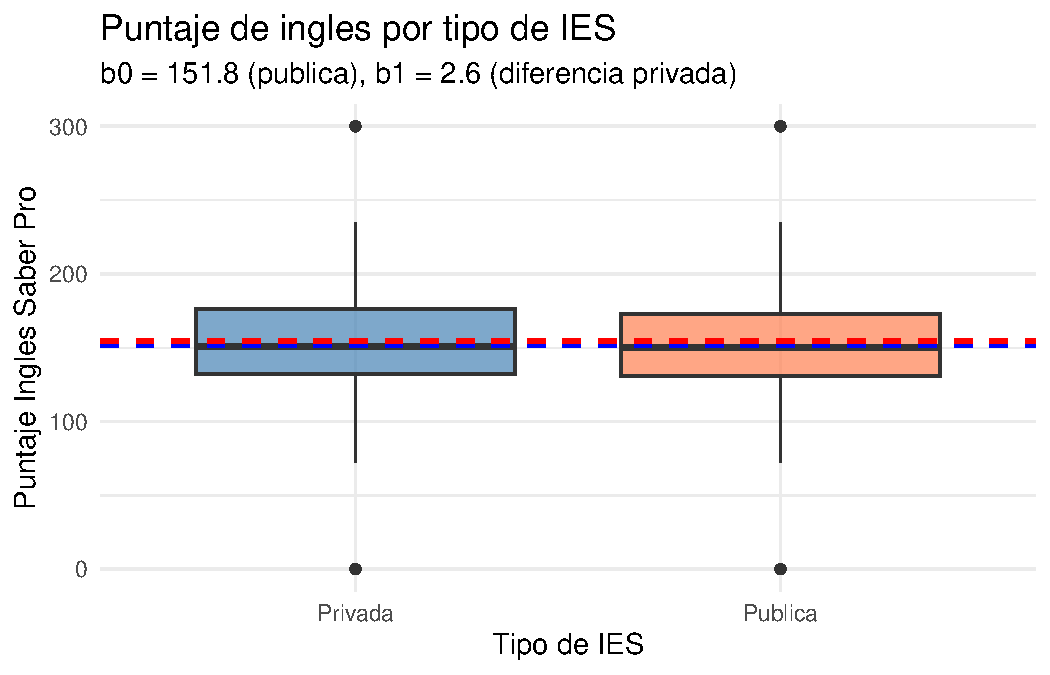
\includegraphics[width=0.85\textwidth]{../S08_chi2_independencia_bondad/figuras/boxplot_dummy.pdf}
\end{center}

\small Las lineas punteadas muestran $\hat{\beta}_0 = 159.59$ (publicas, azul) y $\hat{\beta}_0 + \hat{\beta}_1 = 165.76$ (privadas, rojo). La diferencia es $\hat{\beta}_1 = 6.17$ puntos.
\end{frame}

% --- MULTICOLINEALIDAD PERFECTA ---

\begin{frame}{La trampa de las dummies: multicolinealidad perfecta}
\small
\begin{alertblock}{¿Que pasa si incluimos PRIVADA \textbf{y} PUBLICA?}
\small
Si $\text{PUBLICA} = 1 - \text{PRIVADA}$, entonces PUBLICA es una combinacion lineal exacta de PRIVADA y el intercepto. \textbf{La matriz $\mathbf{X}'\mathbf{X}$ no es invertible} $\Rightarrow$ OLS no tiene solucion.
\end{alertblock}

\vspace{0.2cm}
\textbf{¿Por que?} Con el intercepto (columna de unos), ya sabemos que:
\[
\underbrace{1}_{\text{intercepto}} = \underbrace{\text{PRIVADA}}_{\text{dummy 1}} + \underbrace{\text{PUBLICA}}_{\text{dummy 2}}
\]

La tercera columna es combinacion lineal de las otras dos. El sistema tiene infinitas soluciones: $\beta_0 = 159.59$, $\beta_{\text{PRIV}} = 6.17$, $\beta_{\text{PUB}} = 0$ da lo mismo que $\beta_0 = 165.76$, $\beta_{\text{PRIV}} = 0$, $\beta_{\text{PUB}} = -6.17$.

\vspace{0.2cm}
\textbf{Regla:} para $k$ categorias, usar $k - 1$ dummies. La categoria omitida es el \textbf{grupo de referencia}.
\end{frame}

\begin{frame}[fragile]{Demostracion en R: R elimina la dummy redundante}
\begin{lstlisting}[basicstyle=\ttfamily\scriptsize]
# Crear ambas dummies
saber_pro$PUBLICA <- 1 - saber_pro$PRIVADA

# Intentar incluir ambas
modelo_trap <- lm(MOD_INGLES_PUNT ~ PRIVADA + PUBLICA,
                  data = saber_pro)
summary(modelo_trap)

# Coefficients: (1 not defined because of singularities)
#             Estimate Std. Error t value Pr(>|t|)
# (Intercept)  159.59       0.17  934.75   <2e-16 ***
# PRIVADA        6.17       0.21   29.95   <2e-16 ***
# PUBLICA          NA         NA      NA       NA
\end{lstlisting}

\vspace{0.2cm}
\begin{alertblock}{R detecta el problema}
\small R automaticamente elimina \texttt{PUBLICA} y muestra \texttt{NA}. El mensaje ``\texttt{1 not defined because of singularities}'' significa: hay \textbf{multicolinealidad perfecta}. $(\mathbf{X}'\mathbf{X})^{-1}$ no existe.
\end{alertblock}
\end{frame}

\begin{frame}[fragile]{Otro ejemplo: puntaje global como suma de componentes}
\small
\begin{lstlisting}[basicstyle=\ttfamily\scriptsize]
# Si PUNT_GLOBAL = PUNT_MAT + PUNT_INGLES + PUNT_LECTURA + ...
# entonces incluir PUNT_GLOBAL junto con sus componentes
# genera multicolinealidad perfecta

modelo_mc <- lm(MOD_INGLES_PUNT ~ PUNT_GLOBAL +
                PUNT_MATEMATICAS + PUNT_INGLES,
                data = saber_pro)

# Coefficients: (1 not defined because of singularities)
# R omite una variable porque es combinacion
# lineal de las demas
\end{lstlisting}

\vspace{0.2cm}
\begin{block}{¿Cuando ocurre multicolinealidad perfecta?}
\begin{itemize}\setlength{\itemsep}{2pt}
  \item Incluir \textbf{todas} las dummies de una categoria + intercepto
  \item Incluir una variable que es \textbf{suma/promedio} de otras que ya estan en el modelo
  \item Una variable es transformacion lineal exacta de otra ($X_2 = 3X_1 + 5$)
\end{itemize}
\end{block}
\end{frame}

% ============================================================================
\section{Tablas de regresion en investigacion real}
% ============================================================================

\begin{frame}{¿Como se ven las regresiones en articulos de economia?}
\small
En cualquier articulo de economia van a encontrar \textbf{tablas de regresion} como esta. Saber leerlas es tan fundamental como leer estados financieros en contabilidad.

\vspace{0.2cm}
\begin{block}{Anatomia de una tabla de regresion}
\begin{itemize}\setlength{\itemsep}{2pt}
  \item \textbf{Columnas} = distintos modelos (especificaciones)
  \item \textbf{Filas} = variables independientes
  \item \textbf{Coeficientes} con errores estandar en parentesis
  \item \textbf{Estrellitas} = nivel de significancia
  \item \textbf{Al final}: $N$, $R^2$, controles, efectos fijos
\end{itemize}
\end{block}

\vspace{0.2cm}
Veamos ejemplos de investigaciones reales en economia.
\end{frame}

\begin{frame}{Ejemplo clasico: la ecuacion de Mincer (1974)}
\small
Uno de los modelos mas influyentes en economia laboral:
\[
\ln(\text{salario}_i) = \beta_0 + \beta_1 \cdot \text{Educacion}_i + \beta_2 \cdot \text{Experiencia}_i + \beta_3 \cdot \text{Experiencia}_i^2 + \varepsilon_i
\]

\vspace{0.1cm}
\begin{center}
\footnotesize
\begin{tabular}{lcc}
\toprule
& (1) & (2) \\
& ln(salario) & ln(salario) \\
\midrule
A\~nos de educacion & 0.070*** & 0.085*** \\
& (0.003) & (0.004) \\
Experiencia & & 0.041*** \\
& & (0.002) \\
Experiencia$^2$ & & $-$0.0007*** \\
& & (0.00005) \\
Intercepto & 6.12*** & 5.48*** \\
& (0.04) & (0.05) \\
\midrule
$R^2$ & 0.18 & 0.31 \\
$N$ & 15{,}000 & 15{,}000 \\
\bottomrule
\end{tabular}
\end{center}
\footnotesize Errores estandar en parentesis. *** p $< 0.001$.

\vspace{0.1cm}
\small $\hat{\beta}_1 = 0.085$: cada a\~no adicional de educacion aumenta el salario en $\approx$8.5\%. $R^2 = 0.31$: solo explica 31\% pero el efecto es robusto.
\end{frame}

\begin{frame}{Ejemplo real: efecto de carreteras en educacion (Polanco-Jimenez)}
\small
\textbf{Paper:} ``Road to the Future'' --- impacto de concesiones viales (PPP) en puntajes de Saber 11 en Colombia, usando diferencias en diferencias.

\vspace{0.1cm}
\begin{center}
\scriptsize
\begin{tabular}{lcccc}
\toprule
& 0\% & 10\% & 50\% & 100\% \\
& construido & construido & construido & construido \\
\midrule
\textbf{Puntaje Matematicas (SD)} & $-$0.111* & $-$0.025 & 0.034 & \textbf{0.169**} \\
& (0.050) & (0.051) & (0.031) & (0.032) \\[3pt]
\textbf{Puntaje Lectura (SD)} & $-$0.040 & 0.013 & 0.007 & \textbf{0.112*} \\
& (0.032) & (0.029) & (0.012) & (0.031) \\
\midrule
$N$ & 118{,}143 & 97{,}020 & 89{,}949 & 70{,}535 \\
Efectos fijos & \multicolumn{4}{c}{Colegio + A\~no} \\
SE cluster & \multicolumn{4}{c}{Colegio, Via} \\
\bottomrule
\end{tabular}
\end{center}
\footnotesize SE en parentesis. ** $p<0.01$, * $p<0.05$.

\vspace{0.1cm}
\small \textbf{Lectura:} al 0\% de construccion hay efecto \textbf{negativo} en matematicas (disrupcion). Al 100\%, efecto \textbf{positivo} de 0.17 SD. Dummies de progreso de obra: 4 columnas = 4 modelos.
\end{frame}

\begin{frame}{Ejemplo real: chatbots con IA y aprendizaje (Polanco-Jimenez)}
\small
\textbf{Paper:} ``The Tailoring Premium'' (JEBO, 2025) --- efecto de chatbots genericos vs.\ personalizados en educacion financiera. Experimento aleatorio.

\vspace{0.1cm}
\begin{center}
\scriptsize
\begin{tabular}{lcc}
\toprule
& (1) & (2) \\
& Completo post-test & Ganancia en aprendizaje (SD) \\
\midrule
IA Generica (T1) & $-$0.045** & $-$0.004 \\
& (0.021) & (0.035) \\[3pt]
\textbf{IA Personalizada (T2)} & \textbf{0.097***} & \textbf{0.126***} \\
& (0.021) & (0.037) \\[3pt]
Media grupo control & 0.238 & 0.000 \\
\midrule
$R^2$ & 0.018 & 0.035 \\
$N$ & 2{,}440 & 2{,}440 \\
\bottomrule
\end{tabular}
\end{center}
\footnotesize SE en parentesis. *** $p<0.001$, ** $p<0.01$.

\vspace{0.1cm}
\small \textbf{Lectura:} T1 y T2 son \textbf{dummies} (grupo de referencia = control). La IA personalizada aumenta la probabilidad de completar el test en 9.7 pp y el aprendizaje en 0.13 SD. $R^2 = 0.018$: bajo, pero el efecto es \textbf{causal} (experimento).
\end{frame}

\begin{frame}{¿Como leer una tabla de regresion?}
\small
\begin{enumerate}\setlength{\itemsep}{4pt}
  \item \textbf{Mire la variable dependiente} (arriba de la tabla): ¿que se esta prediciendo?
  \item \textbf{Busque las variables de interes}: ¿cual es el efecto que quiere ver?
  \item \textbf{Lea el coeficiente}: $\hat{\beta}$ = magnitud del efecto
  \item \textbf{Revise las estrellitas}: ¿es significativo?
  \item \textbf{Revise el SE} (en parentesis): ¿la estimacion es precisa?
  \item \textbf{Compare columnas}: ¿el efecto cambia al agregar controles?
  \item \textbf{Mire $R^2$ y $N$}: ¿cuanto explica el modelo? ¿con cuantos datos?
\end{enumerate}

\vspace{0.2cm}
\begin{alertblock}{Se\~nal de alerta}
\small Si el coeficiente cambia mucho entre columnas (al agregar controles), puede haber sesgo por variables omitidas en el modelo simple.
\end{alertblock}
\end{frame}

% --- EJERCICIO LECTURA DE TABLA ---

\begin{frame}{Ejercicio: lea esta tabla (10 min en grupo)}
\small
Un estudio evalua si el acceso a \textbf{internet de alta velocidad} afecta el rendimiento escolar en municipios rurales de Colombia.

\vspace{0.1cm}
\begin{center}
\footnotesize
\begin{tabular}{lccc}
\toprule
& (1) & (2) & (3) \\
& Puntaje Mat & Puntaje Mat & Puntaje Mat \\
\midrule
Internet alta velocidad & 3.42** & 2.89** & 1.05 \\
& (1.21) & (1.15) & (0.98) \\[3pt]
Ingreso per capita & & 0.015*** & 0.012*** \\
& & (0.003) & (0.003) \\[3pt]
Docentes por alumno & & & 12.50*** \\
& & & (2.30) \\[3pt]
\midrule
$R^2$ & 0.04 & 0.08 & 0.15 \\
$N$ & 850 & 850 & 850 \\
\bottomrule
\end{tabular}
\end{center}

\textbf{Preguntas:}
\begin{enumerate}\setlength{\itemsep}{1pt}
  \item ¿Es significativo internet en (1)? ¿En (3)?
  \item ¿Que pasa con el coeficiente de internet entre (1) y (3)?
  \item ¿Que sugiere ese cambio sobre variables omitidas?
  \item ¿Puede concluir que internet \textbf{causa} mejor rendimiento?
\end{enumerate}
\end{frame}

\begin{frame}{Solucion: lectura de la tabla}
\small
\begin{enumerate}\setlength{\itemsep}{3pt}
  \item \textbf{Significancia:} en (1), $t = 3.42/1.21 = 2.83 > 2$ y tiene **, es significativo. En (3), $t = 1.05/0.98 = 1.07 < 2$, \textbf{no es significativo}.

  \item \textbf{El coeficiente baja:} de 3.42 a 1.05. Al agregar controles, el ``efecto'' de internet se reduce un 70\%.

  \item \textbf{Variables omitidas:} los municipios con internet tambien tienen mas ingreso y mas docentes. El modelo (1) atribuia a internet un efecto que en realidad era de esos otros factores. Esto es \textbf{sesgo por variable omitida}: se viola el supuesto de exogeneidad.

  \item \textbf{¿Causalidad?} No. Esto es un estudio observacional. Los municipios que reciben internet no son aleatorios --- probablemente son mas urbanos, mas ricos, con mejor infraestructura educativa. Para causalidad, necesitariamos un RCT o un dise\~no cuasi-experimental (IV, DiD, RDD).
\end{enumerate}

\vspace{0.1cm}
\begin{alertblock}{}
\small Este es el problema central de la econometria: separar correlacion de causalidad. Los supuestos importan.
\end{alertblock}
\end{frame}

\begin{frame}[fragile]{Creemos nuestra propia tabla: 3 modelos con datos ICFES}
\begin{lstlisting}[basicstyle=\ttfamily\scriptsize]
# Modelo 1: solo matematicas
m1 <- lm(MOD_INGLES_PUNT ~ PUNT_MATEMATICAS, data = saber_pro)

# Modelo 2: matematicas + tipo IES
m2 <- lm(MOD_INGLES_PUNT ~ PUNT_MATEMATICAS + PRIVADA,
         data = saber_pro)

# Modelo 3: matematicas + tipo IES + ingles Saber 11
m3 <- lm(MOD_INGLES_PUNT ~ PUNT_MATEMATICAS + PRIVADA +
         PUNT_INGLES, data = saber_pro)

# Comparar coeficientes
coef(summary(m1))["PUNT_MATEMATICAS", ]
coef(summary(m2))["PUNT_MATEMATICAS", ]
coef(summary(m3))["PUNT_MATEMATICAS", ]
\end{lstlisting}

\vspace{0.1cm}
\small ¿Cambia el efecto de matematicas al controlar por tipo de IES e ingles Saber 11?
\end{frame}

\begin{frame}{Nuestra tabla de regresion}
\small
\begin{center}
\begin{tabular}{lccc}
\toprule
& (1) & (2) & (3) \\
& Ingles SP & Ingles SP & Ingles SP \\
\midrule
PUNT\_MATEMATICAS & 1.462*** & 1.430*** & 0.652*** \\
& (0.006) & (0.006) & (0.007) \\[4pt]
PRIVADA & & 4.97*** & 3.56*** \\
& & (0.18) & (0.17) \\[4pt]
PUNT\_INGLES & & & 1.031*** \\
& & & (0.007) \\[4pt]
Intercepto & 76.78*** & 75.12*** & 38.32*** \\
& (0.38) & (0.38) & (0.47) \\
\midrule
$R^2$ & 0.308 & 0.312 & 0.465 \\
$N$ & 125{,}287 & 125{,}287 & 125{,}287 \\
\bottomrule
\end{tabular}
\end{center}
\footnotesize Errores estandar en parentesis. *** p $< 0.001$.

\vspace{0.1cm}
\small \textbf{Observar:} al agregar PUNT\_INGLES (col.\ 3), el efecto de PUNT\_MATEMATICAS \textbf{baja} de 1.46 a 0.65. Parte del ``efecto'' de matematicas era en realidad efecto del ingles de Saber 11. $R^2$ sube de 0.31 a 0.47.
\end{frame}

% ============================================================================
\section{Taller: discriminacion en el mercado laboral (Bertrand \& Mullainathan, 2004)}
% ============================================================================

\begin{frame}{Este paper}
\small

\textcolor{javeriana}{\textbf{Pregunta:}} ¿Existe discriminacion racial en el mercado laboral de Estados Unidos? ¿Los empleadores tratan igual a candidatos blancos y afroamericanos?

\vspace{0.8em}

\textcolor{javeriana}{\textbf{Como:}}
\begin{itemize}\scriptsize\setlength{\itemsep}{1pt}
  \item Un \textit{audit experiment}: enviar CVs \textbf{identicos} a ofertas de empleo reales, variando \textbf{solo el nombre}
  \item 4{,}870 CVs enviados a ofertas en \textbf{Boston y Chicago}
  \item Tratamiento: nombre afroamericano (Lakisha, Jamal) vs.\ nombre blanco (Emily, Greg)
  \item La calidad del CV (alta/baja) tambien fue asignada al azar
\end{itemize}

\vspace{0.5em}

\textcolor{javeriana}{\textbf{Resultados:}}
\begin{itemize}\scriptsize\setlength{\itemsep}{1pt}
  \item Nombres blancos reciben \textbf{50\% mas llamadas}: 9.65\% vs.\ 6.45\%
  \item Un CV de \textbf{alta calidad} beneficia mas a nombres blancos que a nombres afroamericanos
  \item La discriminacion persiste en \textbf{todas} las industrias y ciudades del estudio
\end{itemize}
\end{frame}

\begin{frame}{¿Como se mide la discriminacion?}
\small
\begin{block}{El problema}
\begin{itemize}\setlength{\itemsep}{2pt}
  \item Alguien podria argumentar que las minorias reciben menos llamadas porque tienen \textbf{menos experiencia, menos educacion, peores CVs}
  \item Con datos observacionales, es \textbf{imposible} separar la discriminacion de las diferencias reales en capital humano
  \item Necesitamos un dise\~no que \textbf{aisle} el efecto del nombre
\end{itemize}
\end{block}

\vspace{0.2cm}
\begin{exampleblock}{La solucion: audit experiment (correspondence study)}
\begin{itemize}\setlength{\itemsep}{2pt}
  \item Crear CVs \textbf{identicos} en todo excepto el nombre
  \item Asignar nombres blancos y afroamericanos \textbf{al azar}
  \item Si hay diferencia en callbacks, la \textbf{unica} explicacion es el nombre $\Rightarrow$ discriminacion
\end{itemize}
\end{exampleblock}

\vspace{0.2cm}
\small \textbf{Cita:} Bertrand, M. \& Mullainathan, S. (2004). ``Are Emily and Greg More Employable than Lakisha and Jamal?'' \textit{American Economic Review}, 94(4), 991--1013. Mas de 6{,}000 citas.
\end{frame}

\begin{frame}{El dise\~no experimental}
\footnotesize
\begin{center}
\begin{tikzpicture}[
  box/.style={draw, rounded corners, minimum width=2.6cm, minimum height=0.8cm, align=center, font=\scriptsize},
  arr/.style={-{Stealth[length=2.5mm]}, thick}
]
\node[box, fill=javeriana!15] (ad) at (0,0) {Oferta de empleo\\real (periodico)};
\node[box, fill=green!15] (white) at (-3.5,-2) {Nombre blanco\\(Emily, Greg)};
\node[box, fill=red!15] (black) at (3.5,-2) {Nombre afroamericano\\(Lakisha, Jamal)};
\node[box, fill=javeriana!10] (out1) at (-3.5,-4) {¿Recibio\\callback?};
\node[box, fill=javeriana!10] (out2) at (3.5,-4) {¿Recibio\\callback?};

\draw[arr] (ad) -- node[left, font=\scriptsize] {Aleatorio} (white);
\draw[arr] (ad) -- node[right, font=\scriptsize] {Aleatorio} (black);
\draw[arr] (white) -- node[left, font=\scriptsize] {CV identico} (out1);
\draw[arr] (black) -- node[right, font=\scriptsize] {CV identico} (out2);

\node[font=\scriptsize\bfseries, text=javeriana] at (0,-5) {$\hat{\beta}_1 = P(\text{callback}|\text{blanco}) - P(\text{callback}|\text{afro.})$ = discriminacion};
\end{tikzpicture}
\end{center}
Cada oferta recibe 4 CVs: 2 con nombre blanco, 2 con nombre afroamericano. La calidad (alta/baja) se asigna al azar dentro de cada grupo.
\end{frame}

\begin{frame}{Los nombres del estudio}
\footnotesize
\begin{columns}[T]
\begin{column}{0.48\textwidth}
\begin{block}{Nombres blancos}
\scriptsize
\textbf{Mujeres:} Allison, Anne, Carrie, Emily, Jill, Kristen, Laurie, Meredith, Sarah

\vspace{1pt}
\textbf{Hombres:} Brad, Brendan, Geoffrey, Greg, Jay, Matthew, Neil, Todd
\end{block}
\end{column}

\begin{column}{0.48\textwidth}
\begin{block}{Nombres afroamericanos}
\scriptsize
\textbf{Mujeres:} Aisha, Ebony, Keisha, Kenya, Lakisha, Latonya, Tamika, Tanisha

\vspace{1pt}
\textbf{Hombres:} Darnell, Hakim, Jamal, Jermaine, Kareem, Leroy, Rasheed, Tremayne, Tyrone
\end{block}
\end{column}
\end{columns}

\vspace{0.2cm}
\begin{alertblock}{La brecha en numeros}
\scriptsize Nombres elegidos de registros de nacimiento de Massachusetts e Illinois.
\begin{center}
\scriptsize
\begin{tabular}{lclc}
\toprule
\textbf{Nombre} & \textbf{Callback} & \textbf{Nombre} & \textbf{Callback} \\
\midrule
Brad (blanco) & 15.9\% & Aisha (afro.) & 2.2\% \\
Kristen (blanco) & 13.1\% & Rasheed (afro.) & 3.0\% \\
\bottomrule
\end{tabular}
\end{center}
Brad recibe \textbf{7 veces mas} llamadas que Aisha --- con el \textbf{mismo CV}.
\end{alertblock}
\end{frame}

\begin{frame}{Variables del dataset}
\small
\begin{center}
\footnotesize
\begin{tabular}{llp{7cm}}
\toprule
\textbf{Variable} & \textbf{Tipo} & \textbf{Descripcion} \\
\midrule
\texttt{name} & Factor & Nombre asignado al CV \\
\texttt{ethnicity} & Factor & \texttt{cauc} (blanco) o \texttt{afam} (afroamericano) \\
\texttt{gender} & Factor & \texttt{male} o \texttt{female} \\
\texttt{quality} & Factor & \texttt{high} o \texttt{low} (calidad del CV) \\
\texttt{call} & Factor & \texttt{yes} = recibio llamada, \texttt{no} = no \\
\texttt{city} & Factor & \texttt{boston} o \texttt{chicago} \\
\texttt{experience} & Entera & A\~nos de experiencia en el CV \\
\texttt{honors} & Factor & Si el CV menciona honores academicos \\
\texttt{volunteer} & Factor & Si el CV menciona voluntariado \\
\texttt{college} & Factor & Si el CV incluye titulo universitario \\
\texttt{industry} & Factor & Industria de la oferta de empleo \\
\bottomrule
\end{tabular}
\end{center}

\vspace{0.2cm}
\small \textbf{Nota:} \texttt{call} y \texttt{ethnicity} son factores. Para OLS necesitamos crear dummies numericas (\texttt{callback} y \texttt{afam}).
\end{frame}

\begin{frame}[fragile]{Paso 1: cargar y explorar los datos}
\begin{lstlisting}[basicstyle=\ttfamily\scriptsize]
# --- Cargar datos ---
library(AER)
data(ResumeNames)

# --- Crear variables numericas ---
ResumeNames$callback <- ifelse(
  ResumeNames$call == "yes", 1, 0)
ResumeNames$afam <- ifelse(
  ResumeNames$ethnicity == "afam", 1, 0)

# --- Explorar ---
cat("Observaciones:", nrow(ResumeNames), "\n")  # 4870
table(ResumeNames$ethnicity)
# cauc  afam
# 2435  2435   (perfectamente balanceado)

# Tasa de callback por grupo
aggregate(callback ~ ethnicity,
          data = ResumeNames, FUN = mean)
# cauc: 0.0965   afam: 0.0645
\end{lstlisting}

\vspace{0.1cm}
\small \textbf{Pregunta:} ¿cual es la diferencia en probabilidad de callback? Ese numero es la primera estimacion de discriminacion.
\end{frame}

\begin{frame}[fragile]{Paso 2: verificar la aleatorizacion}
\small
\textbf{Si la aleatorizacion funciono}, la calidad del CV debe estar \textbf{balanceada} entre grupos.

\begin{lstlisting}[basicstyle=\ttfamily\scriptsize]
# --- Balance de calidad por grupo ---
table(ResumeNames$ethnicity, ResumeNames$quality)
#        low  high
# cauc  1212  1223
# afam  1226  1209

# --- Balance de experiencia ---
aggregate(experience ~ ethnicity,
          data = ResumeNames, FUN = mean)

# --- Balance de genero ---
table(ResumeNames$ethnicity, ResumeNames$gender)
\end{lstlisting}

\vspace{0.2cm}
\begin{block}{Preguntas (en grupo, 5 min)}
\begin{enumerate}\setlength{\itemsep}{1pt}
  \item ¿Los CVs de alta calidad estan repartidos igual entre grupos?
  \item ¿Por que es importante verificar esto \textbf{antes} de estimar el efecto?
  \item ¿Que concluyen sobre la aleatorizacion?
\end{enumerate}
\end{block}
\end{frame}

\begin{frame}[fragile]{Paso 3: visualizar}
\begin{lstlisting}[basicstyle=\ttfamily\scriptsize]
library(ggplot2)

# Barplot: tasa de callback por grupo
tasas <- aggregate(callback ~ ethnicity,
                   data = ResumeNames, FUN = mean)
ggplot(tasas, aes(x = ethnicity, y = callback,
                  fill = ethnicity)) +
  geom_col(alpha = 0.8, show.legend = FALSE) +
  scale_fill_manual(values = c("afam" = "#E74C3C",
                               "cauc" = "#3498DB")) +
  labs(x = "Grupo etnico", y = "Tasa de callback",
       title = "Bertrand & Mullainathan (2004)") +
  theme_minimal()

# Callback por nombre (top y bottom 5)
tasas_n <- aggregate(callback ~ name,
                     data = ResumeNames, FUN = mean)
tasas_n <- tasas_n[order(-tasas_n$callback), ]
head(tasas_n, 5)  # Brad, Jay, Kristen...
tail(tasas_n, 5)  # Kareem, Keisha, Rasheed, Aisha
\end{lstlisting}
\end{frame}

\begin{frame}[fragile]{Paso 4: OLS con dummy --- modelo de probabilidad lineal}
\begin{lstlisting}[basicstyle=\ttfamily\scriptsize]
# --- Modelo 1: callback ~ afam ---
m1 <- lm(callback ~ afam, data = ResumeNames)
summary(m1)

# Coefficients:
#             Estimate Std. Error t value Pr(>|t|)
# (Intercept) 0.096509   0.005505  17.53   <2e-16 ***
# afam       -0.032033   0.007785  -4.12  3.9e-05 ***

# Intervalo de confianza
confint(m1)

# Verificar: identico a prueba t
t.test(callback ~ ethnicity, data = ResumeNames,
       var.equal = TRUE)
\end{lstlisting}

\vspace{0.1cm}
\begin{block}{Modelo de Probabilidad Lineal (LPM)}
\small Cuando $Y$ es binaria (0/1), OLS se llama LPM. $\hat{\beta}_1$ se interpreta como \textbf{cambio en la probabilidad}: tener nombre afroamericano \textbf{reduce} la probabilidad de callback en 3.2 puntos porcentuales.
\end{block}
\end{frame}

\begin{frame}{Interpretacion del modelo}
\small
\begin{block}{¿Que significan los coeficientes?}
\begin{itemize}\setlength{\itemsep}{3pt}
  \item $\hat{\beta}_0 = 0.0965$: probabilidad de callback con nombre \textbf{blanco} = 9.65\%
  \item $\hat{\beta}_1 = -0.0320$: tener nombre afroamericano \textbf{reduce} la probabilidad en 3.2 pp
  \item $\hat{\beta}_0 + \hat{\beta}_1 = 0.0645$: probabilidad de callback con nombre \textbf{afroamericano} = 6.45\%
\end{itemize}
\end{block}

\vspace{0.2cm}
\begin{alertblock}{Preguntas (5 min)}
\begin{enumerate}\setlength{\itemsep}{2pt}
  \item ¿$\hat{\beta}_1$ es significativo? Use las 3 formas: $|t| > 2$, p-valor, IC
  \item El IC al 95\% para $\hat{\beta}_1$ es $[-0.047,\; -0.017]$. ¿Contiene al 0?
  \item $-3.2$ pp parece poco. Pero en \textbf{terminos relativos}: $0.032/0.0965 = 33\%$. ¿Que les dice?
  \item ¿Este $\hat{\beta}_1$ es \textbf{causal}? ¿Por que?
\end{enumerate}
\end{alertblock}
\end{frame}

\begin{frame}[fragile]{Paso 5: calcular $R^2$ a mano}
\begin{lstlisting}[basicstyle=\ttfamily\scriptsize]
# --- R^2 paso a paso ---
SST <- sum((ResumeNames$callback -
            mean(ResumeNames$callback))^2)
SSE <- sum(residuals(m1)^2)
SSR <- SST - SSE

cat("SST:", round(SST, 2), "\n")
cat("SSE:", round(SSE, 2), "\n")
cat("SSR:", round(SSR, 2), "\n")
cat("R2 manual:", round(1 - SSE / SST, 4), "\n")
cat("R2 summary:", round(summary(m1)$r.squared, 4), "\n")
# R2 = 0.0035
\end{lstlisting}

\vspace{0.1cm}
\begin{alertblock}{Preguntas}
\footnotesize
\begin{enumerate}\setlength{\itemsep}{1pt}
  \item $R^2 = 0.003$, extremadamente bajo. ¿Eso significa que la discriminacion no existe?
  \item \textbf{No.} Miles de factores determinan un callback (industria, cargo, momento, suerte). El nombre explica poco de la variacion total, pero su efecto es \textbf{real, significativo y causal}.
  \item Recuerden: $R^2$ mide \textbf{prediccion}, no \textbf{causalidad}.
\end{enumerate}
\end{alertblock}
\end{frame}

\begin{frame}[fragile]{Paso 6: agregar covariables --- 4 modelos}
\begin{lstlisting}[basicstyle=\ttfamily\scriptsize]
# Crear dummies adicionales
RN <- ResumeNames
RN$high_q   <- ifelse(RN$quality == "high", 1, 0)
RN$female   <- ifelse(RN$gender == "female", 1, 0)
RN$chicago  <- ifelse(RN$city == "chicago", 1, 0)

m2 <- lm(callback ~ afam + high_q, data = RN)
m3 <- lm(callback ~ afam + high_q + experience +
         female, data = RN)
m4 <- lm(callback ~ afam + high_q + experience +
         female + chicago, data = RN)

cat("=== Efecto de nombre afroamericano ===\n")
cat("M1:", round(coef(m1)["afam"], 4), "\n")
cat("M2:", round(coef(m2)["afam"], 4), "\n")
cat("M3:", round(coef(m3)["afam"], 4), "\n")
cat("M4:", round(coef(m4)["afam"], 4), "\n")
\end{lstlisting}

\vspace{0.1cm}
\small \textbf{Observe:} el coeficiente de \texttt{afam} \textbf{apenas cambia} ($\approx -0.032$) al agregar controles. Eso confirma que la aleatorizacion funciono.
\end{frame}

\begin{frame}[fragile]{Paso 6 (cont.): comparar $R^2$ e intervalos de confianza}
\begin{lstlisting}[basicstyle=\ttfamily\scriptsize]
# R-squared
cat("=== R-squared ===\n")
cat("M1:", round(summary(m1)$r.squared, 4), "\n")
cat("M2:", round(summary(m2)$r.squared, 4), "\n")
cat("M3:", round(summary(m3)$r.squared, 4), "\n")
cat("M4:", round(summary(m4)$r.squared, 4), "\n\n")

# Intervalos de confianza para afam
cat("=== IC 95% para discriminacion ===\n")
ic1 <- confint(m1)["afam", ]
ic4 <- confint(m4)["afam", ]
cat("M1:", round(ic1, 4), "\n")
cat("M4:", round(ic4, 4), "\n")
\end{lstlisting}

\vspace{0.1cm}
\begin{block}{Preguntas clave (10 min en grupo)}
\footnotesize
\begin{enumerate}\setlength{\itemsep}{1pt}
  \item ¿Cambio $\hat{\beta}_{\text{afam}}$ entre M1 y M4? ¿Por que?
  \item ¿Que paso con el $R^2$? ¿Por que sigue tan bajo?
  \item ¿Por que en un RCT el coeficiente \textbf{no deberia} cambiar? Conecte con exogeneidad.
  \item ¿Se estrecharon los IC? ¿Que implica?
\end{enumerate}
\end{block}
\end{frame}

\begin{frame}{Paso 7: nuestra tabla de regresion}
\footnotesize
\begin{center}
\scriptsize
\renewcommand{\arraystretch}{1.2}
\begin{tabular}{lcccc}
\toprule
& (1) & (2) & (3) & (4) \\
& callback & callback & callback & callback \\
\midrule
afam & $-$0.0320*** & $-$0.0320*** & $-$0.0320*** & $-$0.0321*** \\
& (0.0078) & (0.0078) & (0.0078) & (0.0078) \\[3pt]
high\_quality & & 0.0141 & 0.0112 & 0.0119 \\
& & (0.0078) & (0.0078) & (0.0078) \\[3pt]
experience & & & 0.0032*** & 0.0026*** \\
& & & (0.0008) & (0.0008) \\[3pt]
female & & & 0.0079 & 0.0175 \\
& & & (0.0092) & (0.0096) \\[3pt]
chicago & & & & $-$0.0288*** \\
& & & & (0.0083) \\
\midrule
$R^2$ & 0.0035 & 0.0041 & 0.0078 & 0.0102 \\
$N$ & 4{,}870 & 4{,}870 & 4{,}870 & 4{,}870 \\
\bottomrule
\end{tabular}
\end{center}
\footnotesize Errores estandar en parentesis. *** $p < 0.001$.

\vspace{0.1cm}
\tiny \textbf{Observe:} $\hat{\beta}_{\text{afam}} \approx -0.032$ \textbf{no cambia} en las 4 columnas. La aleatorizacion garantiza exogeneidad: agregar controles no afecta el efecto causal. Chicago tiene 2.9 pp menos callbacks que Boston.
\end{frame}

\begin{frame}[fragile]{Paso 8: ¿la calidad del CV ayuda igual a todos?}
\small
El hallazgo mas impactante del paper: mejorar el CV beneficia \textbf{mas a los blancos}.

\begin{lstlisting}[basicstyle=\ttfamily\scriptsize]
# --- Interaccion: afam x calidad ---
m_int <- lm(callback ~ afam * high_quality,
            data = ResumeNames)
summary(m_int)

# afam:high_quality  -> efecto diferencial

# Callback por grupo y calidad
aggregate(callback ~ ethnicity + quality,
          data = ResumeNames, FUN = mean)
#  ethnicity quality   callback
#  cauc      low       0.0835
#  cauc      high      0.1095
#  afam      low       0.0629
#  afam      high      0.0661
\end{lstlisting}

\vspace{0.1cm}
\begin{alertblock}{Implicacion de politica publica}
\small Para nombres blancos, un CV de alta calidad sube el callback de 8.4\% a 11.0\% (+2.6 pp). Para nombres afroamericanos, apenas sube de 6.3\% a 6.6\% (+0.3 pp). \textbf{Invertir en mejor CV no reduce la brecha}. La discriminacion es \textbf{estructural}.
\end{alertblock}
\end{frame}

\begin{frame}{Reflexion: ¿que aprendimos con Bertrand \& Mullainathan?}
\small
\begin{exampleblock}{Conexiones con la teoria}
\begin{itemize}\setlength{\itemsep}{3pt}
  \item \textbf{Dummy}: \texttt{afam} es una dummy. $\hat{\beta}_1$ mide la \textbf{diferencia en probabilidad} de callback --- lo mismo que un \texttt{t.test()}
  \item \textbf{LPM}: OLS con $Y$ binaria = modelo de probabilidad lineal. $\hat{\beta}$ = cambio en probabilidad
  \item \textbf{$R^2$}: $0.003$, extremadamente bajo, pero el efecto es \textbf{causal y significativo}. $R^2$ mide prediccion, no causalidad
  \item \textbf{Covariables en RCT}: agregar controles \textbf{no cambia} $\hat{\beta}_1$ (exogeneidad por dise\~no)
  \item \textbf{Interaccion}: la brecha no desaparece con mejor CV. La discriminacion es \textbf{estructural}
\end{itemize}
\end{exampleblock}

\vspace{0.2cm}
\begin{alertblock}{La leccion del paper}
\small Un nombre en un CV no deberia importar. Pero importa. Este paper demostro con evidencia \textbf{experimental} que la discriminacion racial existe en el mercado laboral --- y que no basta con ``mejorar el CV''. La econometria rigurosa cambia el debate de opiniones a \textbf{evidencia}.
\end{alertblock}
\end{frame}

\begin{frame}{Conexion con Colombia y el mundo}
\small
\begin{block}{La discriminacion no es solo de EE.UU.}
Los audit experiments se han replicado en todo el mundo:
\begin{itemize}\setlength{\itemsep}{2pt}
  \item \textbf{Colombia:} estudios en Bogota muestran diferencias en callbacks por apellidos, color de piel, y estrato socioeconomico
  \item \textbf{Europa:} nombres arabes vs.\ europeos en Francia, Suecia, Alemania, y Pa\'ises Bajos --- resultados similares
  \item \textbf{Genero:} Goldin \& Rouse (2000, \textit{AER}) mostraron que audiciones ciegas aumentaron la contratacion de mujeres en orquestas sinfonicas
\end{itemize}
\end{block}

\vspace{0.2cm}
\begin{alertblock}{Para sus carreras}
\small Si van a evaluar politicas de inclusion, programas de empleo, o practicas de contratacion, las herramientas de hoy ($R^2$, significancia, dummies, interacciones, dise\~no experimental) son \textbf{exactamente} lo que van a usar.
\end{alertblock}
\end{frame}

% ============================================================================
\section{Resumen y proxima sesion}
% ============================================================================

\begin{frame}{Resumen de la sesion}
\footnotesize
\begin{block}{$R^2$ y significancia}
\begin{itemize}\setlength{\itemsep}{0pt}
  \item $R^2 = \text{SSR}/\text{SST}$: proporcion de variacion explicada
  \item Prueba t: $t = \hat{\beta}/\text{SE}(\hat{\beta})$. Si $|t| > 2$: significativo al 5\%
  \item p-valor, IC y prueba t dicen lo mismo de diferente forma
\end{itemize}
\end{block}

\begin{block}{Dummies y multicolinealidad}
\begin{itemize}\setlength{\itemsep}{0pt}
  \item Dummy = OLS para comparar grupos ($k$ categorias $\Rightarrow$ $k-1$ dummies)
  \item Multicolinealidad perfecta: R omite la variable redundante (NA)
\end{itemize}
\end{block}

\begin{block}{Taller Bertrand \& Mullainathan (2004)}
\begin{itemize}\setlength{\itemsep}{0pt}
  \item En un RCT, la dummy de tratamiento captura el efecto causal (discriminacion)
  \item Modelo de probabilidad lineal (LPM): OLS con $Y$ binaria = cambio en probabilidad
  \item $R^2 = 0.003$ pero el efecto es significativo y causal
  \item Agregar covariables en un RCT mejora precision sin cambiar el efecto
\end{itemize}
\end{block}
\end{frame}

\begin{frame}{Proxima sesion (S10)}
\begin{exampleblock}{Regresion lineal multiple}
$Y_i = \beta_0 + \beta_1 X_{1i} + \beta_2 X_{2i} + \cdots + \beta_k X_{ki} + \varepsilon_i$

\vspace{0.2cm}
\begin{itemize}\setlength{\itemsep}{3pt}
  \item Predecir controlando por multiples variables simultaneamente
  \item Ceteris paribus: el efecto de $X_1$ \textbf{manteniendo constantes} $X_2, \ldots, X_k$
  \item $R^2$ ajustado: penalizar por agregar variables
  \item Multicolinealidad imperfecta: VIF
\end{itemize}
\end{exampleblock}
\end{frame}

\begin{frame}
\begin{center}
\Large
Gracias

\vspace{1cm}
\normalsize
Preguntas y discusion
\end{center}
\end{frame}

\end{document}
